%%% Latex Template for PhD Dissertation, MEAM Department @UPenn
%%% Created By : Morteza H. Siboni (hakimi1364@gmail.com)
%%% Based on   : the Dissertation templated available at https : //www.math.upenn.edu/grad/thesisstyle.html
%%% 
%%% ***IMPORTANT***
%%% please consult university of Pennsylvania Doctoral Dissertation Manual (http://www.upenn.edu/grad/DissManual.html) for consistency.  

\documentclass[12pt]{report}

%%%%%%%%%%%%%%%%%%%%
%%% Font Related Packages 
\usepackage{amsmath}
\usepackage{amssymb}
\usepackage{amsthm}
\usepackage{amsfonts}
\usepackage{MnSymbol}
%%% Graphics Related Packages 
\usepackage[dvips]{graphicx}
\usepackage{psfrag}
\usepackage[usenames]{color}
\usepackage[small]{subfigure}
\usepackage[percent]{overpic}
%%% Table Related Packages
\usepackage{stmaryrd}
\usepackage{multirow}
\usepackage{dcolumn}% Align table columns on decimal point
\usepackage[table]{xcolor}
%%% Bibliography Related Packages
\usepackage{natbib}
%%% Hyper-link settings and package [optional]
\definecolor{gray1}{gray}{0.2}
\definecolor{gray2}{gray}{0.4}
\usepackage{hyperref}
\hypersetup{
    %bookmarks=true,         % show bookmarks bar?
    unicode=false,          % non-Latin characters in Acrobat’s bookmarks
    pdftoolbar=true,        % show Acrobat’s toolbar?
    pdfmenubar=true,        % show Acrobat’s menu?
    pdffitwindow=true,     % window fit to page when opened
    pdfstartview={FitH},    % fits the width of the page to the window
    pdftitle={TITLE, optional},    % title
    pdfauthor={AUTHOR, optional},     % author
    pdfsubject={Subject},   % subject of the document
    pdfcreator={Creator},   % creator of the document
    pdfproducer={Producer}, % producer of the document
    pdfkeywords={KEYWORDS, optional}, % list of keywords
    pdfnewwindow=true,      % links in new window
    colorlinks = true,       % false: boxed links; true: colored links
    linkcolor=	gray2,          % color of internal links
    citecolor=	gray2,        % color of links to bibliography
    filecolor=	gray2,      % color of file links
    urlcolor=	gray2,           % color of external links
    breaklinks = true
}
%%% Additional Packages 
\usepackage{bm}% bold math
\usepackage{leftidx}
%\usepackage{showkeys} % shows the keys [Use this to show the latex labels in the final pdf for ease of access] [comment it out for the final verstion]
%%%%%%%%%%%%%%%%%%%%


%% folders containing the figures and plots
%% **for example each folder can contain all the figures corresponding to a specific paper
%% **add more folders as necessary 
\graphicspath{ {./figs_set_1/}
               {./figs_set_2/} 
             }


%% make sure that the margins comply with the dissertation guild line (** this is very important)
\usepackage{geometry}
\geometry{letterpaper, 
          left     = 1.5in,
          right    = 1.0in,
          top      = 1.0in,
          bottom   = 1.0in,
          footskip = 0.2in}


\usepackage{caption, setspace}
\captionsetup[table]{font={stretch=1.0}}     %% change 1.0 as you like
\captionsetup[figure]{font={stretch=1.0}}    %% change 1.0 as you like


\usepackage[notbib]{tocbibind}


\pagestyle{plain}
\newcommand{\doublespaced}{\renewcommand{\baselinestretch}{1.5}\normalfont}
\newcommand{\singlespaced}{\renewcommand{\baselinestretch}{1.0}\normalfont}
\newcommand{\draftspaced}{\singlespaced} %for draft only 
%\newcommand{\draftspaced}{\doublespaced} %for final version

%%%%%\theoremstyle{plain}
%%%%\newtheorem{theorem}{Theorem}[section]
%%%%\newtheorem{corollary}[theorem]{Corollary}
%%%%%\newtheorem*{main}{Main~Theorem}
%%%%\newtheorem{lemma}[theorem]{Lemma}
%%%%\newtheorem{proposition}[theorem]{Proposition}
%%%%
%%%%
%%%%\theoremstyle{definition}
%%%%\newtheorem{definition}[theorem]{Definition}
%%%%
%%%%
%%%%\theoremstyle{remark}
%%%%\newtheorem{remark}[theorem]{Remark}
%%%%\newtheorem{example}[theorem]{Example}


%%%\newcommand{\f}{\mathfrak}
%%%\newcommand{\mb}{\mathbb}
%%%\newcommand{\mr}{\mathrm}
%%%\newcommand{\mf}{\mathbf}
%%%\newcommand{\mc}{\mathcal}
%%%\newcommand{\e}{\emph}
%%%\newcommand{\vp}{\varphi}
%%%\newcommand{\Diff}{\textrm{Diff}}
%%%\newcommand{\Norm}{\textrm{Norm}}
%%%\newcommand{\Hom}{\textrm{Hom}}
%%%\newcommand{\ch}{\textrm{char}}
%%%\newcommand{\lcm}{\textrm{lcm}}
%%%%\newcommand{\ca}{\mathcal}
%%%\newcommand{\wt}{\widetilde}
%%%%\newcommand{\ol}{\overline}

%%%%%%%%%%%%%%%%%%%%%%
%%% BEGIN COSTUMIZED COMMANDS
%%% add your command here
%%% End COSTUMIZED COMMANDS
%%%%%%%%%%%%%%%%%%%%%%

%%%% NUMBERINGS
%%%% EQS
\numberwithin{equation}{chapter}
%%%% FOOTNOTES
\usepackage{chngcntr}
\counterwithout{footnote}{chapter}


\doublespaced
\def\thetitle{TITLE OF THE THESIS GOES HERE}
\def\theauthor{John Smith}   
\def\theadvisor{Jane Doe}
\def\THEAUTHOR  {}      
\def\THEADVISOR {} 
\def\theyear{yyyy}


\begin{document}

\pagenumbering{roman}
\doublespaced
\large\newlength{\oldparskip}\setlength\oldparskip{\parskip}\parskip=0.0in
\thispagestyle{empty}
\begin{center}
%\vspace*{\fill}
\thetitle

\vspace*{20pt}

\begin{small}

\theauthor

\vspace*{20pt}

A DISSERTATION 

in 

Mechanical Engineering and Applied Mechanics 

Presented to the Faculties of the University of Pennsylvania

in

Partial Fulfillment of the Requirements for the 

Degree of Doctor of Philosophy

\theyear

\end{small}

\end{center}

\vspace{45pt}

\begin{small}
\singlespaced
\noindent Supervisor of Dissertation:  \\ \\ \\
\noindent \rule[1ex]{3in}{0.3mm}  \\
\noindent Jane Doe, Professor \\
Department of Mechanical Engineering and Applied Mechanics\\ \\ 

\noindent Graduate Group Chairperson: \\ \\ \\
\noindent \rule[1ex]{3in}{0.3mm} \\
\noindent Jack London, Associate Professor \\
Department of Mechanical Engineering and Applied Mechanics \\

\vspace*{15pt}


\singlespaced
\noindent Dissertation Committee: \\
\noindent Jane Doe, Professor \\
Department of Mechanical Engineering and Applied Mechanics \\

\noindent Emily Black, Associate Professor \\
Department of Mechanical Engineering and Applied Mechanics\\

\end{small}

\vspace*{\fill}

\normalsize\parskip=\oldparskip


\newpage
\doublespaced

%\chapter*{Copyright Notice}
\thispagestyle{empty}

\vspace*{150pt}

\begin{center}
\begin{minipage}[b]{0.75\textwidth}
\begin{center}
\textbf{TITLE OF THE THESIS GOES HERE}

\vspace*{10pt}

\textbf{COPYRIGHT}

\vspace*{10pt}

\textbf{20nn}

\vspace*{10pt}

\textbf{John Smith}
\end{center}
\end{minipage}
\end{center}


%%% Dedications 
\newpage
\vspace*{150pt}
\begin{Large}
\begin{center}
\textit{To Somebody}
\end{center}
\end{Large}

%%% Acknolegements
\newpage
\chapter*{Acknowledgments}


The completion of my PhD would not have been possible without the support and guidance of the following people. It is to them that I owe my deepest gratitude.

Thanks a lot of people here!!!

\newpage
%\vspace*{\fill}
\begin{center}
ABSTRACT\\
\vspace{0.25in}
\thetitle\\
\vspace{0.25in}
\theauthor\\
\theadvisor \\
\vspace{0.25in}
\end{center}

\singlespaced
\noindent Lorem Ipsum is simply dummy text of the printing and typesetting industry. Lorem Ipsum has been the industry's standard dummy text ever since the 1500s, when an unknown printer took a galley of type and scrambled it to make a type specimen book. It has survived not only five centuries, but also the leap into electronic typesetting, remaining essentially unchanged. It was popularised in the 1960s with the release of Letraset sheets containing Lorem Ipsum passages, and more recently with desktop publishing software like Aldus PageMaker including versions of Lorem Ipsum.

\vspace*{15pt}
\noindent Aenean malesuada tincidunt quam, ut dapibus nunc fermentum porta. Donec euismod auctor laoreet. Pellentesque euismod enim et orci tempor, eget posuere nisi aliquet. Integer posuere tristique sem eu vehicula. Integer eget odio et mauris tincidunt viverra. Donec euismod tortor congue magna lacinia, ac accumsan arcu dignissim. Cras non diam eget mi ultricies laoreet quis eu odio. Suspendisse eu iaculis erat, at ornare nisi. Etiam ut neque ligula. Nam luctus orci a nulla vulputate, eget vestibulum nunc vulputate. Quisque at arcu auctor, maximus velit pretium, pulvinar nisi. In eu finibus augue. Aliquam ligula diam, tempus id nibh at, condimentum convallis quam. Sed a leo non tortor aliquam venenatis.

\vspace*{15pt}
\noindent Nunc tempus dolor eget posuere consectetur. In hac habitasse platea dictumst. Phasellus leo ligula, tristique non libero at, facilisis varius quam. Sed a finibus diam. Mauris elementum maximus enim, ut dictum odio ornare non. Nulla accumsan sem ante, sit amet consequat augue imperdiet id. Nam in rutrum elit. Praesent viverra sem ac urna cursus, in tempus arcu accumsan. Duis quis tristique est, ut pellentesque enim. Nulla tempor egestas facilisis. Praesent auctor justo est, ut blandit ligula placerat non. Donec ut quam dui.  


\vspace*{\fill}

\newpage

\singlespaced
\tableofcontents


\newpage

\singlespaced
\listoftables


\newpage

\singlespaced
\listoffigures


\newpage

%%%
%%%\newpage
%%%\listoftodos

\doublespaced
\pagenumbering{arabic}

%\include{introdept}
%\include{back}
%\include{finitedept}
%\include{infinitedept}
%
%
%%%%%% Introduction
\chapter{Introduction}

Lorem ipsum dolor sit amet, consectetur adipiscing elit. Donec aliquet dui tincidunt ligula placerat faucibus nec at neque. Sed et accumsan magna, dictum vehicula ipsum. Praesent faucibus nisi metus, sed bibendum lacus sagittis a. Suspendisse enim tellus, pellentesque a tristique in, gravida eu risus. Aenean vitae rhoncus tellus. Suspendisse potenti. Etiam quis quam ultrices, sodales felis eu, fringilla ante. Vestibulum nec purus tellus. Suspendisse id euismod nunc. Nulla ultricies pretium auctor. Nam posuere nec eros in pharetra. Pellentesque mattis accumsan erat, vitae malesuada eros efficitur eu. Nullam dui nulla, porttitor eu sapien varius, condimentum iaculis urna \cite{B76}.

Integer consequat efficitur convallis. Vivamus et semper libero, sit amet vestibulum nisi. Vestibulum eget justo ut tellus tincidunt tincidunt sit amet et turpis. Nulla finibus nulla a enim sollicitudin pretium. Phasellus quis iaculis lorem. Integer a nisi consequat, venenatis diam a, condimentum risus. Nulla condimentum, mi sed mattis tincidunt, nulla nisl facilisis elit, vitae facilisis arcu augue ut lectus. Morbi finibus enim et erat tempor dignissim. Fusce dolor magna, ultrices ac eros et, fermentum congue orci. Praesent dictum, mi vel suscipit feugiat, justo ligula porta odio, sed placerat enim felis pulvinar nibh. Ut sodales, nulla congue feugiat fringilla, velit neque feugiat urna, ac dapibus mi ex eu felis. Aliquam nunc nisl, pellentesque auctor posuere in, lobortis eget arcu. Ut sed nisl imperdiet, porta risus eget, bibendum turpis. Aliquam vel auctor magna.

Nunc tempus dolor eget posuere consectetur. In hac habitasse platea dictumst. Phasellus leo ligula, tristique non libero at, facilisis varius quam. Sed a finibus diam. Mauris elementum maximus enim, ut dictum odio ornare non. Nulla accumsan sem ante, sit amet consequat augue imperdiet id. Nam in rutrum elit. Praesent viverra sem ac urna cursus, in tempus arcu accumsan. Duis quis tristique est, ut pellentesque enim. Nulla tempor egestas facilisis. Praesent auctor justo est, ut blandit ligula placerat non. Donec ut quam dui.

Donec imperdiet dui in laoreet pellentesque. Pellentesque dictum gravida turpis, vitae congue urna. Nulla facilisi. Aliquam ut nisl sagittis, posuere nulla eget, posuere leo. Etiam nec quam laoreet, lacinia elit ac, porttitor orci. Ut blandit dignissim quam, sed viverra risus faucibus et. Nunc convallis tempus varius. Ut pulvinar euismod rhoncus. Aliquam sit amet nisl sed diam malesuada rutrum. Morbi quis volutpat ipsum, finibus pretium neque. Suspendisse ut semper quam. In eu mauris congue, iaculis sapien a, mollis dui. Vivamus varius consequat pharetra. Donec quis lorem quis tortor lacinia ultrices. Praesent commodo odio quis leo tincidunt laoreet.

Aenean malesuada tincidunt quam, ut dapibus nunc fermentum porta. Donec euismod auctor laoreet. Pellentesque euismod enim et orci tempor, eget posuere nisi aliquet. Integer posuere tristique sem eu vehicula. Integer eget odio et mauris tincidunt viverra. Donec euismod tortor congue magna lacinia, ac accumsan arcu dignissim. Cras non diam eget mi ultricies laoreet quis eu odio. Suspendisse eu iaculis erat, at ornare nisi. Etiam ut neque ligula. Nam luctus orci a nulla vulputate, eget vestibulum nunc vulputate. Quisque at arcu auctor, maximus velit pretium, pulvinar nisi. In eu finibus augue. Aliquam ligula diam, tempus id nibh at, condimentum convallis quam. Sed a leo non tortor aliquam venenatis \cite{L67}. 

%%% you may or may not choose to divide your dissertation into parts
%%% if you do not wish to divide your thesis into parts comment out everything that is in between ''%% BEGINNING OF PART PAGE'' and ''%% END OF PART PAGE'' below and every where else in the document.
%% BEGINNING OF PART PAGE
\part*{Part I: Title}
\addcontentsline{toc}{part}{Part I: Title}
\addtocontents{toc}{\protect\mbox{}\protect\hrulefill\par}
%% END OF PART PAGE

%%% include chapters below
\chapter{chapter 1 title}

Aenean malesuada tincidunt quam, ut dapibus nunc fermentum porta. Donec euismod auctor laoreet. Pellentesque euismod enim et orci tempor, eget posuere nisi aliquet. Integer posuere tristique sem eu vehicula. Integer eget odio et mauris tincidunt viverra. Donec euismod tortor congue magna lacinia, ac accumsan arcu dignissim. Cras non diam eget mi ultricies laoreet quis eu odio. Suspendisse eu iaculis erat, at ornare nisi. Etiam ut neque ligula. Nam luctus orci a nulla vulputate, eget vestibulum nunc vulputate. Quisque at arcu auctor, maximus velit pretium, pulvinar nisi. In eu finibus augue. Aliquam ligula diam, tempus id nibh at, condimentum convallis quam. Sed a leo non tortor aliquam venenatis.


\section{sec 1}
Aenean malesuada tincidunt quam, ut dapibus nunc fermentum porta. Donec euismod auctor laoreet. Pellentesque euismod enim et orci tempor, eget posuere nisi aliquet. Integer posuere tristique sem eu vehicula. Integer eget odio et mauris tincidunt viverra. Donec euismod tortor congue magna lacinia, ac accumsan arcu dignissim. Cras non diam eget mi ultricies laoreet quis eu odio. Suspendisse eu iaculis erat, at ornare nisi. Etiam ut neque ligula. Nam luctus orci a nulla vulputate, eget vestibulum nunc vulputate. Quisque at arcu auctor, maximus velit pretium, pulvinar nisi. In eu finibus augue. Aliquam ligula diam, tempus id nibh at, condimentum convallis quam. Sed a leo non tortor aliquam venenatis.

\section{sec 2}
Aenean malesuada tincidunt quam, ut dapibus nunc fermentum porta. Donec euismod auctor laoreet. Pellentesque euismod enim et orci tempor, eget posuere nisi aliquet. Integer posuere tristique sem eu vehicula. Integer eget odio et mauris tincidunt viverra. Donec euismod tortor congue magna lacinia, ac accumsan arcu dignissim. Cras non diam eget mi ultricies laoreet quis eu odio. Suspendisse eu iaculis erat, at ornare nisi. Etiam ut neque ligula. Nam luctus orci a nulla vulputate, eget vestibulum nunc vulputate. Quisque at arcu auctor, maximus velit pretium, pulvinar nisi. In eu finibus augue. Aliquam ligula diam, tempus id nibh at, condimentum convallis quam. Sed a leo non tortor aliquam venenatis.

...

Figure \ref{sample1} shows lab lab lah
\begin{figure}[ph!]
\psfrag{XL}[][][0.75][0]{$x$}
\psfrag{YL}[][][0.75][0]{$y$}
\psfrag{S1}[][][0.75][0]{a circle}
\psfrag{S2}[][][0.75][0]{a star}
\centering
\subfigure[]{\label{} 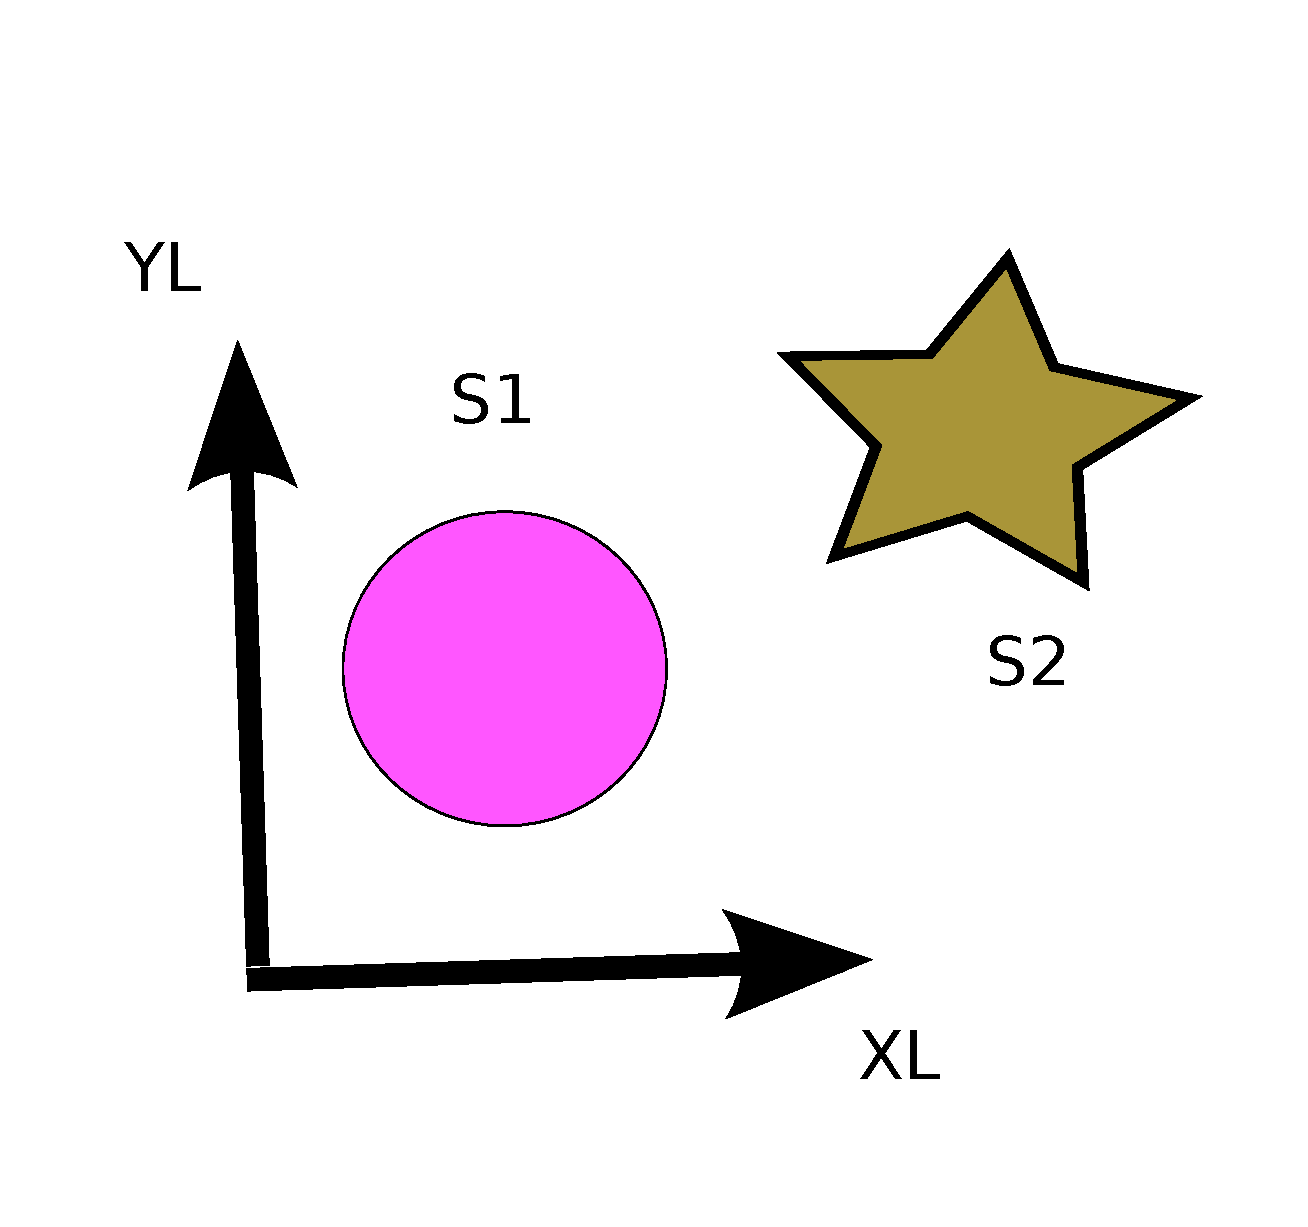
\includegraphics[width=0.35\textwidth]{paper_1_fig_1}}
\subfigure[]{\label{} 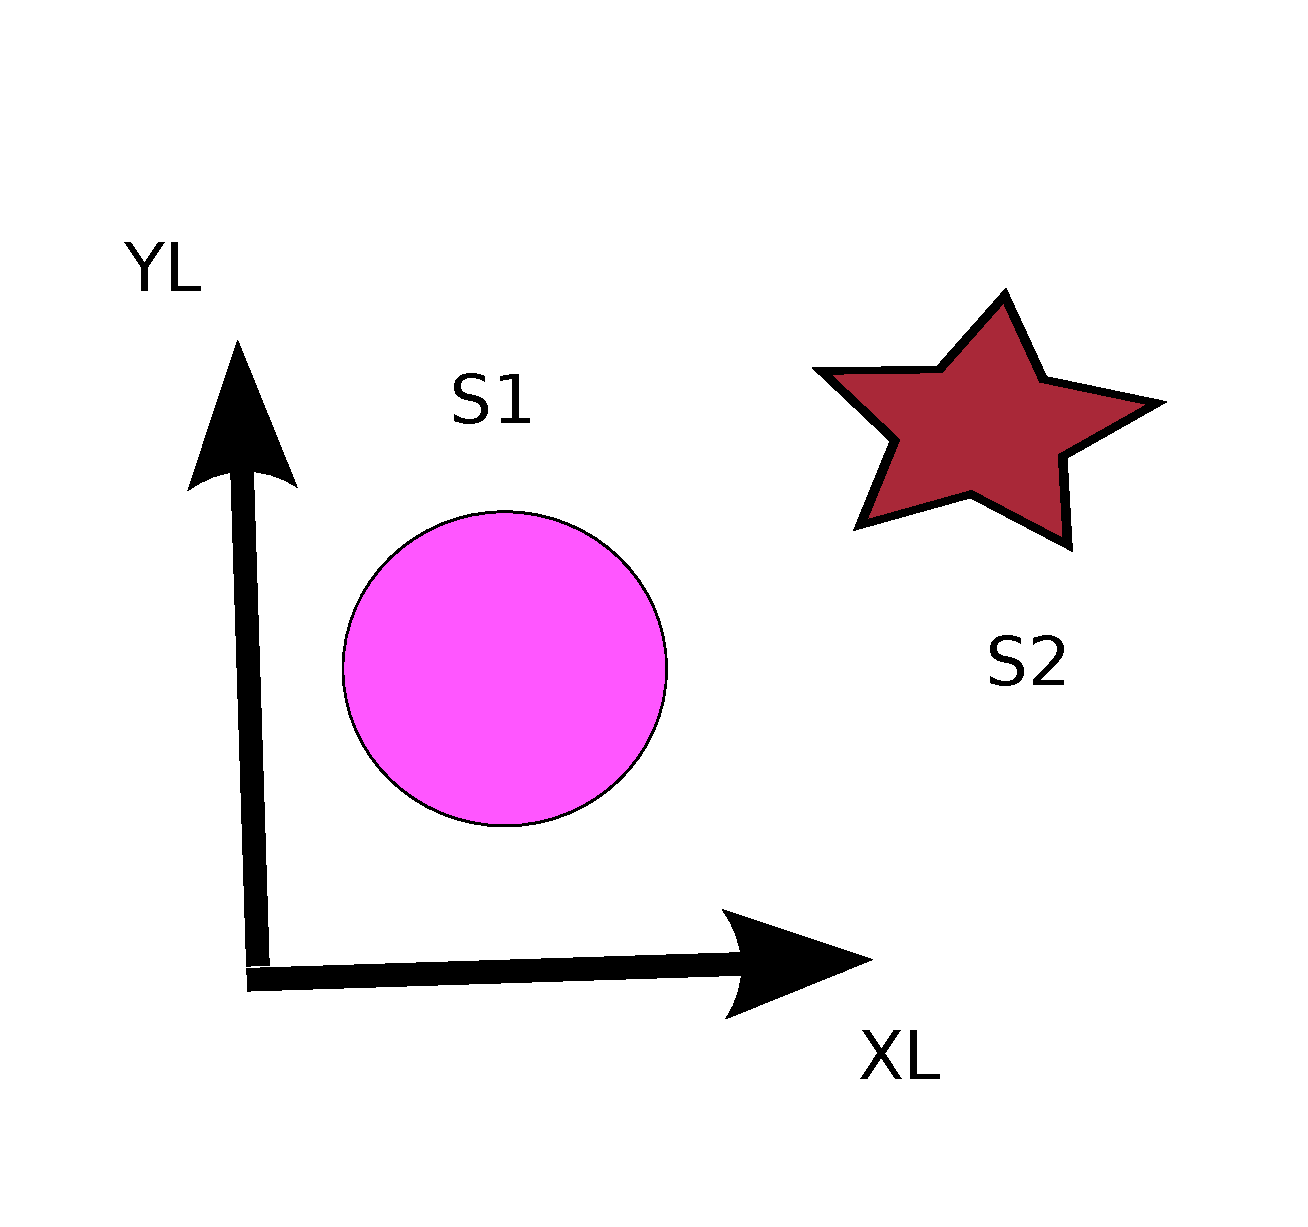
\includegraphics[width=0.35\textwidth]{paper_1_fig_2}} \\
\caption{\label{sample1} This is a sample figure that uses the ``psfrag'' package [https://en.wikipedia.org/wiki/PSfrag]. This package is very useful because it can replace predefined labels in the eps figures with latex commands. The only draw-back is that it does not work with pdfLatex. So to get a final pdf you have to make a ps first and then convert it to pdf {the steps to this are latex->dvi2ps->ps2pdf}. Usually the implementation of the latex come from executables for doing the operations shown in the curly braces. (a) shows something and (b) shows something else.} 
\end{figure}


Figure \ref{sample2} is another figure sample 
\begin{figure}[ph!]
\centering
\subfigure[]{\label{} 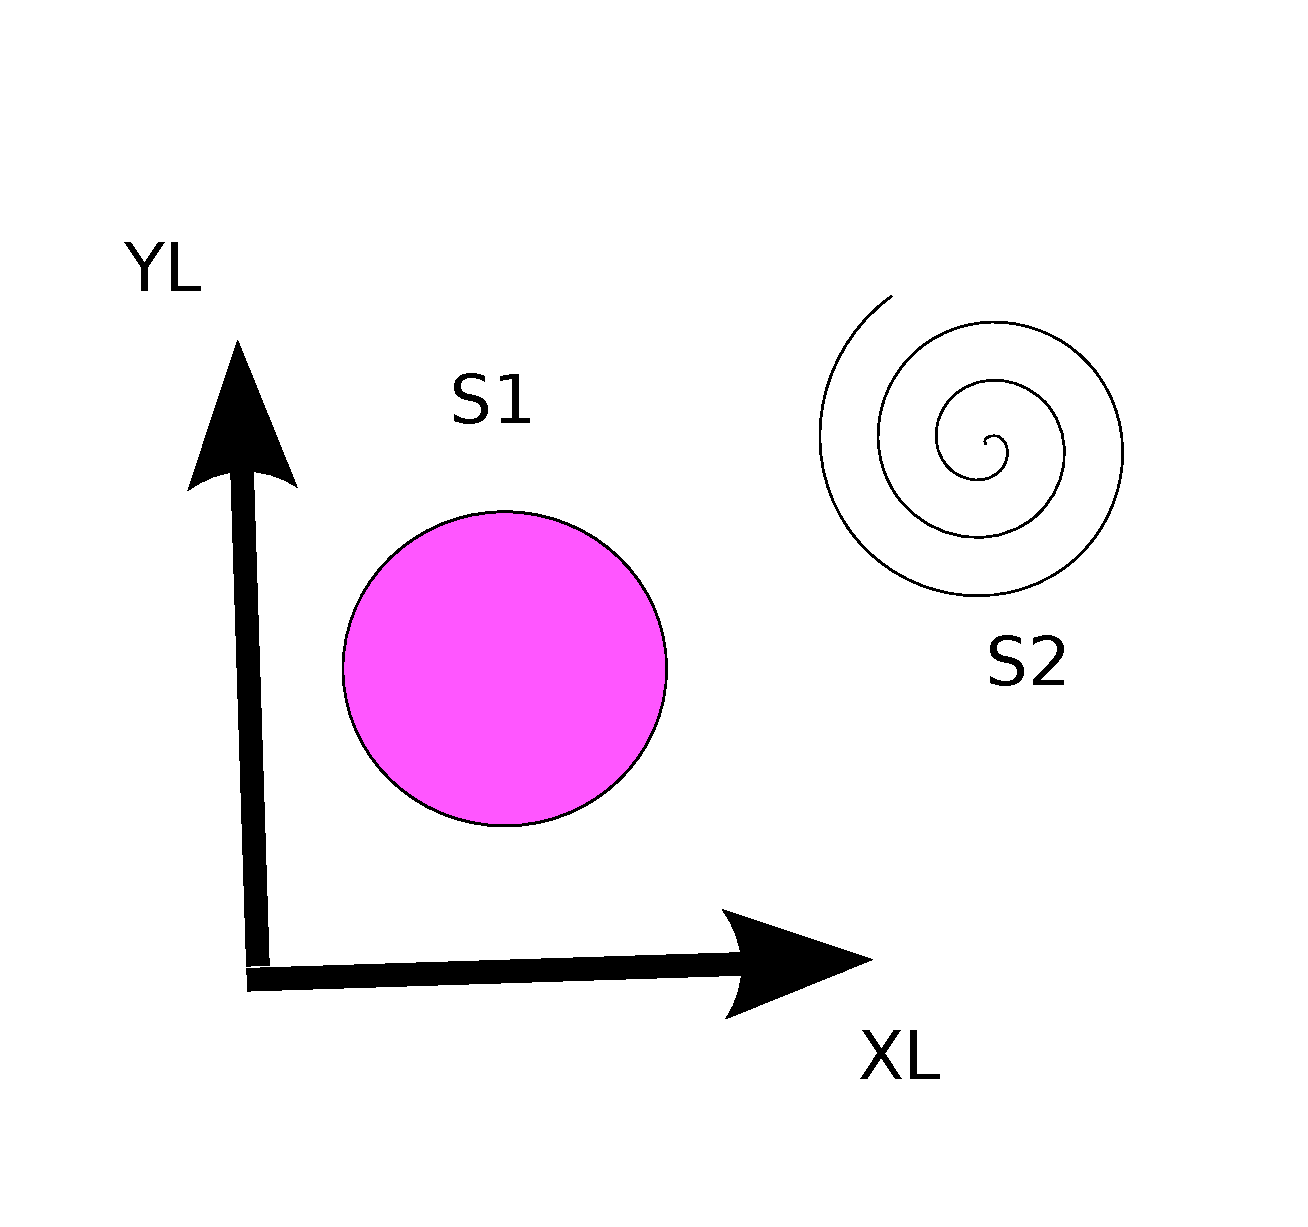
\includegraphics[width=0.35\textwidth]{paper_2_fig_1}}
\subfigure[]{\label{} 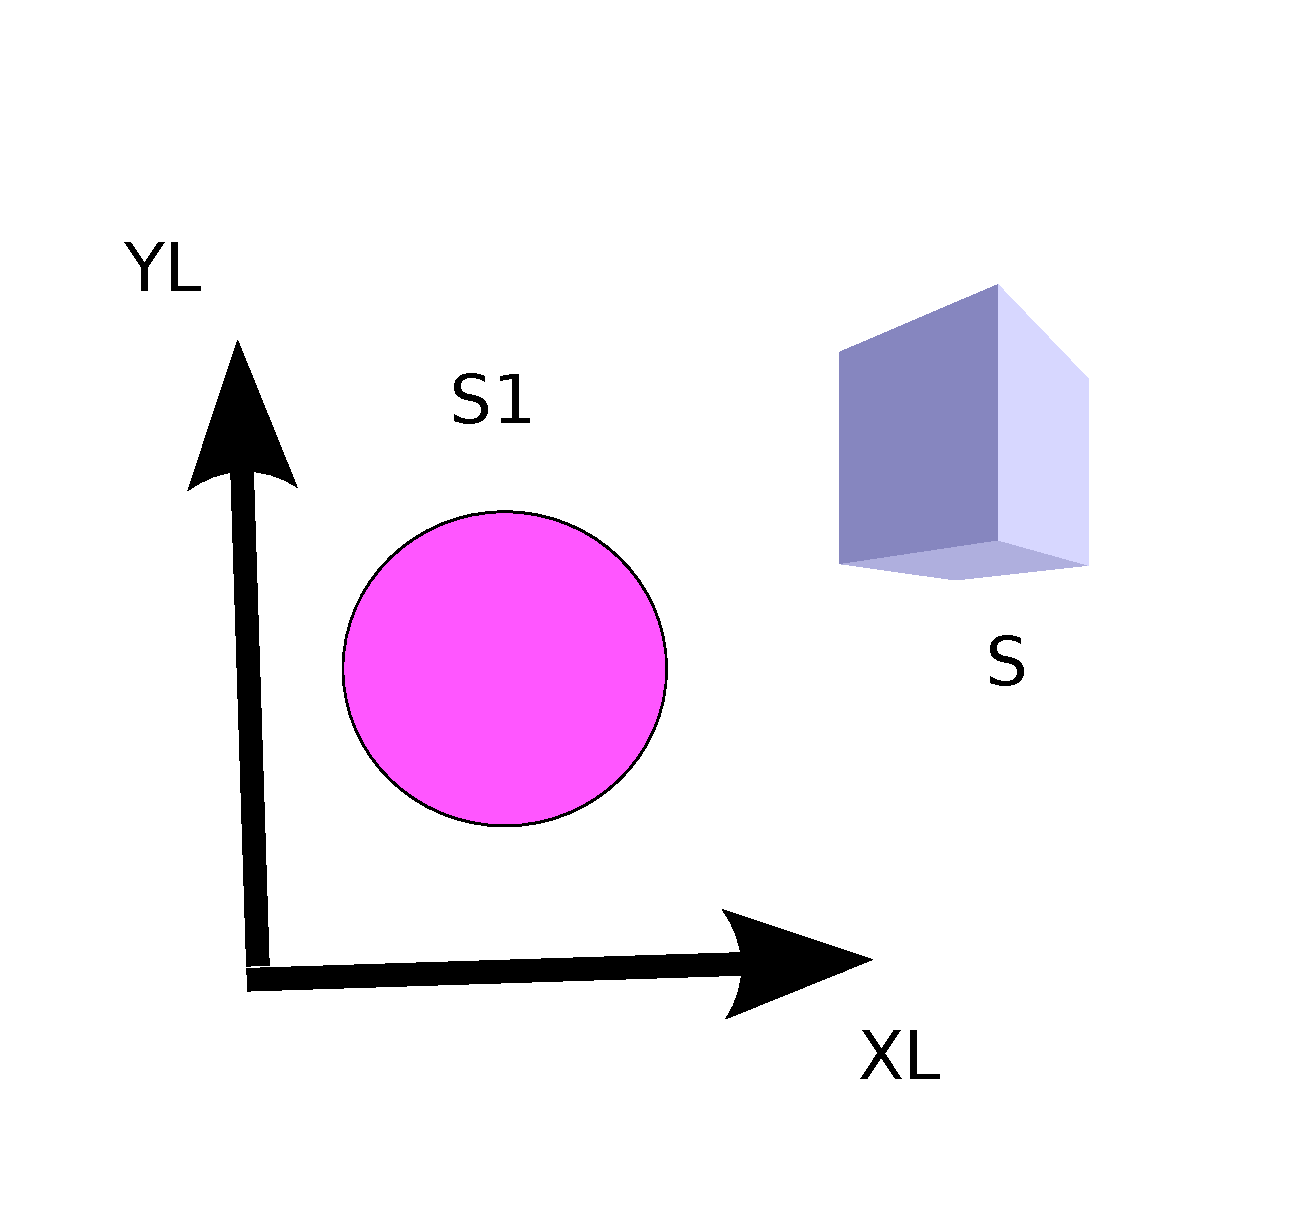
\includegraphics[width=0.35\textwidth]{paper_2_fig_2}} \\
\caption{\label{sample1} This is a sample figure that does not use the ``psfrag'' package [https://en.wikipedia.org/wiki/PSfrag], and therefore original labels in the eps files are shown. (Note that you can open the eps files with a text editor and search for the corresponding labels in it, and changes the labels, if you want to, form within the eps file.)  a) shows something and (b) shows something else.} 
\end{figure}



\chapter{chapter 2 title}

Aenean malesuada tincidunt quam, ut dapibus nunc fermentum porta. Donec euismod auctor laoreet. Pellentesque euismod enim et orci tempor, eget posuere nisi aliquet. Integer posuere tristique sem eu vehicula. Integer eget odio et mauris tincidunt viverra. Donec euismod tortor congue magna lacinia, ac accumsan arcu dignissim. Cras non diam eget mi ultricies laoreet quis eu odio. Suspendisse eu iaculis erat, at ornare nisi. Etiam ut neque ligula. Nam luctus orci a nulla vulputate, eget vestibulum nunc vulputate. Quisque at arcu auctor, maximus velit pretium, pulvinar nisi. In eu finibus augue. Aliquam ligula diam, tempus id nibh at, condimentum convallis quam. Sed a leo non tortor aliquam venenatis.


\section{sec 1}
Aenean malesuada tincidunt quam, ut dapibus nunc fermentum porta. Donec euismod auctor laoreet. Pellentesque euismod enim et orci tempor, eget posuere nisi aliquet. Integer posuere tristique sem eu vehicula. Integer eget odio et mauris tincidunt viverra. Donec euismod tortor congue magna lacinia, ac accumsan arcu dignissim. Cras non diam eget mi ultricies laoreet quis eu odio. Suspendisse eu iaculis erat, at ornare nisi. Etiam ut neque ligula. Nam luctus orci a nulla vulputate, eget vestibulum nunc vulputate. Quisque at arcu auctor, maximus velit pretium, pulvinar nisi. In eu finibus augue. Aliquam ligula diam, tempus id nibh at, condimentum convallis quam. Sed a leo non tortor aliquam venenatis.

\section{sec 2}
Aenean malesuada tincidunt quam, ut dapibus nunc fermentum porta. Donec euismod auctor laoreet. Pellentesque euismod enim et orci tempor, eget posuere nisi aliquet. Integer posuere tristique sem eu vehicula. Integer eget odio et mauris tincidunt viverra. Donec euismod tortor congue magna lacinia, ac accumsan arcu dignissim. Cras non diam eget mi ultricies laoreet quis eu odio. Suspendisse eu iaculis erat, at ornare nisi. Etiam ut neque ligula. Nam luctus orci a nulla vulputate, eget vestibulum nunc vulputate. Quisque at arcu auctor, maximus velit pretium, pulvinar nisi. In eu finibus augue. Aliquam ligula diam, tempus id nibh at, condimentum convallis quam. Sed a leo non tortor aliquam venenatis.

...

%%% add more parts and chapters if you wish
%% BEGINNING OF PART PAGE
\part*{Part II: Title}
\addcontentsline{toc}{part}{Part II: Title}
\addtocontents{toc}{\protect\mbox{}\protect\hrulefill\par}
%% END OF PART PAGE

%% add more chapters

%%% Conclusion
\chapter{Closure}


Lorem ipsum dolor sit amet, consectetur adipiscing elit. Donec aliquet dui tincidunt ligula placerat faucibus nec at neque. Sed et accumsan magna, dictum vehicula ipsum. Praesent faucibus nisi metus, sed bibendum lacus sagittis a. Suspendisse enim tellus, pellentesque a tristique in, gravida eu risus. Aenean vitae rhoncus tellus. Suspendisse potenti. Etiam quis quam ultrices, sodales felis eu, fringilla ante. Vestibulum nec purus tellus. Suspendisse id euismod nunc. Nulla ultricies pretium auctor. Nam posuere nec eros in pharetra. Pellentesque mattis accumsan erat, vitae malesuada eros efficitur eu. Nullam dui nulla, porttitor eu sapien varius, condimentum iaculis urna.

Integer consequat efficitur convallis. Vivamus et semper libero, sit amet vestibulum nisi. Vestibulum eget justo ut tellus tincidunt tincidunt sit amet et turpis. Nulla finibus nulla a enim sollicitudin pretium. Phasellus quis iaculis lorem. Integer a nisi consequat, venenatis diam a, condimentum risus. Nulla condimentum, mi sed mattis tincidunt, nulla nisl facilisis elit, vitae facilisis arcu augue ut lectus. Morbi finibus enim et erat tempor dignissim. Fusce dolor magna, ultrices ac eros et, fermentum congue orci. Praesent dictum, mi vel suscipit feugiat, justo ligula porta odio, sed placerat enim felis pulvinar nibh. Ut sodales, nulla congue feugiat fringilla, velit neque feugiat urna, ac dapibus mi ex eu felis. Aliquam nunc nisl, pellentesque auctor posuere in, lobortis eget arcu. Ut sed nisl imperdiet, porta risus eget, bibendum turpis. Aliquam vel auctor magna.

Nunc tempus dolor eget posuere consectetur. In hac habitasse platea dictumst. Phasellus leo ligula, tristique non libero at, facilisis varius quam. Sed a finibus diam. Mauris elementum maximus enim, ut dictum odio ornare non. Nulla accumsan sem ante, sit amet consequat augue imperdiet id. Nam in rutrum elit. Praesent viverra sem ac urna cursus, in tempus arcu accumsan. Duis quis tristique est, ut pellentesque enim. Nulla tempor egestas facilisis. Praesent auctor justo est, ut blandit ligula placerat non. Donec ut quam dui.

Donec imperdiet dui in laoreet pellentesque. Pellentesque dictum gravida turpis, vitae congue urna. Nulla facilisi. Aliquam ut nisl sagittis, posuere nulla eget, posuere leo. Etiam nec quam laoreet, lacinia elit ac, porttitor orci. Ut blandit dignissim quam, sed viverra risus faucibus et. Nunc convallis tempus varius. Ut pulvinar euismod rhoncus. Aliquam sit amet nisl sed diam malesuada rutrum. Morbi quis volutpat ipsum, finibus pretium neque. Suspendisse ut semper quam. In eu mauris congue, iaculis sapien a, mollis dui. Vivamus varius consequat pharetra. Donec quis lorem quis tortor lacinia ultrices. Praesent commodo odio quis leo tincidunt laoreet.

Aenean malesuada tincidunt quam, ut dapibus nunc fermentum porta. Donec euismod auctor laoreet. Pellentesque euismod enim et orci tempor, eget posuere nisi aliquet. Integer posuere tristique sem eu vehicula. Integer eget odio et mauris tincidunt viverra. Donec euismod tortor congue magna lacinia, ac accumsan arcu dignissim. Cras non diam eget mi ultricies laoreet quis eu odio. Suspendisse eu iaculis erat, at ornare nisi. Etiam ut neque ligula. Nam luctus orci a nulla vulputate, eget vestibulum nunc vulputate. Quisque at arcu auctor, maximus velit pretium, pulvinar nisi. In eu finibus augue. Aliquam ligula diam, tempus id nibh at, condimentum convallis quam. Sed a leo non tortor aliquam venenatis.

%%%Appendices
\part*{Appendix}
\addcontentsline{toc}{part}{Appendix}
\addtocontents{toc}{\protect\mbox{}\protect\hrulefill\par}

\appendix
\chapter{appendix title}

Lorem ipsum dolor sit amet, consectetur adipiscing elit. Donec aliquet dui tincidunt ligula placerat faucibus nec at neque. Sed et accumsan magna, dictum vehicula ipsum. Praesent faucibus nisi metus, sed bibendum lacus sagittis a. Suspendisse enim tellus, pellentesque a tristique in, gravida eu risus. Aenean vitae rhoncus tellus. Suspendisse potenti. Etiam quis quam ultrices, sodales felis eu, fringilla ante. Vestibulum nec purus tellus. Suspendisse id euismod nunc. Nulla ultricies pretium auctor. Nam posuere nec eros in pharetra. Pellentesque mattis accumsan erat, vitae malesuada eros efficitur eu. Nullam dui nulla, porttitor eu sapien varius, condimentum iaculis urna.

Integer consequat efficitur convallis. Vivamus et semper libero, sit amet vestibulum nisi. Vestibulum eget justo ut tellus tincidunt tincidunt sit amet et turpis. Nulla finibus nulla a enim sollicitudin pretium. Phasellus quis iaculis lorem. Integer a nisi consequat, venenatis diam a, condimentum risus. Nulla condimentum, mi sed mattis tincidunt, nulla nisl facilisis elit, vitae facilisis arcu augue ut lectus. Morbi finibus enim et erat tempor dignissim. Fusce dolor magna, ultrices ac eros et, fermentum congue orci. Praesent dictum, mi vel suscipit feugiat, justo ligula porta odio, sed placerat enim felis pulvinar nibh. Ut sodales, nulla congue feugiat fringilla, velit neque feugiat urna, ac dapibus mi ex eu felis. Aliquam nunc nisl, pellentesque auctor posuere in, lobortis eget arcu. Ut sed nisl imperdiet, porta risus eget, bibendum turpis. Aliquam vel auctor magna.

Nunc tempus dolor eget posuere consectetur. In hac habitasse platea dictumst. Phasellus leo ligula, tristique non libero at, facilisis varius quam. Sed a finibus diam. Mauris elementum maximus enim, ut dictum odio ornare non. Nulla accumsan sem ante, sit amet consequat augue imperdiet id. Nam in rutrum elit. Praesent viverra sem ac urna cursus, in tempus arcu accumsan. Duis quis tristique est, ut pellentesque enim. Nulla tempor egestas facilisis. Praesent auctor justo est, ut blandit ligula placerat non. Donec ut quam dui.

Donec imperdiet dui in laoreet pellentesque. Pellentesque dictum gravida turpis, vitae congue urna. Nulla facilisi. Aliquam ut nisl sagittis, posuere nulla eget, posuere leo. Etiam nec quam laoreet, lacinia elit ac, porttitor orci. Ut blandit dignissim quam, sed viverra risus faucibus et. Nunc convallis tempus varius. Ut pulvinar euismod rhoncus. Aliquam sit amet nisl sed diam malesuada rutrum. Morbi quis volutpat ipsum, finibus pretium neque. Suspendisse ut semper quam. In eu mauris congue, iaculis sapien a, mollis dui. Vivamus varius consequat pharetra. Donec quis lorem quis tortor lacinia ultrices. Praesent commodo odio quis leo tincidunt laoreet.

Aenean malesuada tincidunt quam, ut dapibus nunc fermentum porta. Donec euismod auctor laoreet. Pellentesque euismod enim et orci tempor, eget posuere nisi aliquet. Integer posuere tristique sem eu vehicula. Integer eget odio et mauris tincidunt viverra. Donec euismod tortor congue magna lacinia, ac accumsan arcu dignissim. Cras non diam eget mi ultricies laoreet quis eu odio. Suspendisse eu iaculis erat, at ornare nisi. Etiam ut neque ligula. Nam luctus orci a nulla vulputate, eget vestibulum nunc vulputate. Quisque at arcu auctor, maximus velit pretium, pulvinar nisi. In eu finibus augue. Aliquam ligula diam, tempus id nibh at, condimentum convallis quam. Sed a leo non tortor aliquam venenatis.

\addtocontents{toc}{\protect\setcounter{tocdepth}{0}}
\chapter{another appendix title}

Lorem ipsum dolor sit amet, consectetur adipiscing elit. Donec aliquet dui tincidunt ligula placerat faucibus nec at neque. Sed et accumsan magna, dictum vehicula ipsum. Praesent faucibus nisi metus, sed bibendum lacus sagittis a. Suspendisse enim tellus, pellentesque a tristique in, gravida eu risus. Aenean vitae rhoncus tellus. Suspendisse potenti. Etiam quis quam ultrices, sodales felis eu, fringilla ante. Vestibulum nec purus tellus. Suspendisse id euismod nunc. Nulla ultricies pretium auctor. Nam posuere nec eros in pharetra. Pellentesque mattis accumsan erat, vitae malesuada eros efficitur eu. Nullam dui nulla, porttitor eu sapien varius, condimentum iaculis urna.

Integer consequat efficitur convallis. Vivamus et semper libero, sit amet vestibulum nisi. Vestibulum eget justo ut tellus tincidunt tincidunt sit amet et turpis. Nulla finibus nulla a enim sollicitudin pretium. Phasellus quis iaculis lorem. Integer a nisi consequat, venenatis diam a, condimentum risus. Nulla condimentum, mi sed mattis tincidunt, nulla nisl facilisis elit, vitae facilisis arcu augue ut lectus. Morbi finibus enim et erat tempor dignissim. Fusce dolor magna, ultrices ac eros et, fermentum congue orci. Praesent dictum, mi vel suscipit feugiat, justo ligula porta odio, sed placerat enim felis pulvinar nibh. Ut sodales, nulla congue feugiat fringilla, velit neque feugiat urna, ac dapibus mi ex eu felis. Aliquam nunc nisl, pellentesque auctor posuere in, lobortis eget arcu. Ut sed nisl imperdiet, porta risus eget, bibendum turpis. Aliquam vel auctor magna.

Nunc tempus dolor eget posuere consectetur. In hac habitasse platea dictumst. Phasellus leo ligula, tristique non libero at, facilisis varius quam. Sed a finibus diam. Mauris elementum maximus enim, ut dictum odio ornare non. Nulla accumsan sem ante, sit amet consequat augue imperdiet id. Nam in rutrum elit. Praesent viverra sem ac urna cursus, in tempus arcu accumsan. Duis quis tristique est, ut pellentesque enim. Nulla tempor egestas facilisis. Praesent auctor justo est, ut blandit ligula placerat non. Donec ut quam dui.

Donec imperdiet dui in laoreet pellentesque. Pellentesque dictum gravida turpis, vitae congue urna. Nulla facilisi. Aliquam ut nisl sagittis, posuere nulla eget, posuere leo. Etiam nec quam laoreet, lacinia elit ac, porttitor orci. Ut blandit dignissim quam, sed viverra risus faucibus et. Nunc convallis tempus varius. Ut pulvinar euismod rhoncus. Aliquam sit amet nisl sed diam malesuada rutrum. Morbi quis volutpat ipsum, finibus pretium neque. Suspendisse ut semper quam. In eu mauris congue, iaculis sapien a, mollis dui. Vivamus varius consequat pharetra. Donec quis lorem quis tortor lacinia ultrices. Praesent commodo odio quis leo tincidunt laoreet.

Aenean malesuada tincidunt quam, ut dapibus nunc fermentum porta. Donec euismod auctor laoreet. Pellentesque euismod enim et orci tempor, eget posuere nisi aliquet. Integer posuere tristique sem eu vehicula. Integer eget odio et mauris tincidunt viverra. Donec euismod tortor congue magna lacinia, ac accumsan arcu dignissim. Cras non diam eget mi ultricies laoreet quis eu odio. Suspendisse eu iaculis erat, at ornare nisi. Etiam ut neque ligula. Nam luctus orci a nulla vulputate, eget vestibulum nunc vulputate. Quisque at arcu auctor, maximus velit pretium, pulvinar nisi. In eu finibus augue. Aliquam ligula diam, tempus id nibh at, condimentum convallis quam. Sed a leo non tortor aliquam venenatis.


\addtocontents{toc}{\protect\setcounter{tocdepth}{3}}



%% The Bibliography [the agsm style needs to be installed in your implementation of the latex (texlive) or (miktex)]
\addcontentsline{toc}{part}{Bibliography}
%%%Bibliography
\bibliographystyle{agsm}
\bibliography{bb_Bibliography} 

\end{document}
